\documentclass[conference]{IEEEtran}
\IEEEoverridecommandlockouts
% The preceding line is only needed to identify funding in the first footnote. If that is unneeded, please comment it out.
\usepackage{cite}
\usepackage{amsmath,amssymb,amsfonts}
\usepackage{algorithmic}
\usepackage{graphicx}
\usepackage{textcomp}
\usepackage{xcolor}
\def\BibTeX{{\rm B\kern-.05em{\sc i\kern-.025em b}\kern-.08em
    T\kern-.1667em\lower.7ex\hbox{E}\kern-.125emX}}

\renewcommand{\figurename}{Gambar}
\renewcommand{\tablename}{Tabel}
\renewcommand{\IEEEkeywordsname}{Keywords}
\usepackage{caption}
\usepackage{pgf}
    
\begin{document}

\title{An Effective Intrusion Detection System using 
Supervised Machine Learning Techniques.\\
%{\footnotesize \textsuperscript{*}Note: Sub-titles are not captured in Xplore and should not be used}
%\thanks{Identify applicable funding agency here. If none, delete this.}
}

\author{\IEEEauthorblockN{Muhammad Ali Imron}
\IEEEauthorblockA{\textit{Faculty of Information Technology} \\
\textit{Institut Teknologi Batam}\\
Batam, Indonesia \\
1822007@student.iteba.ac.id}
}

\maketitle

\begin{abstract}
Dengan meningkatnya penggunaan sumber daya Internet, penyerang dunia maya menggunakan cara baru untuk menyerang layanan jaringan. Dengan demikian keamanan jaringan menjadi bagian tak terelakkan dari sistem jaringan. Untuk mendeteksi serangan tersebut secara efisien dan efektif, IDS yang kuat (Sistem Deteksi Intrusi) diperlukan. IDS adalah alat yang menganalisis setiap paket secara mendalam untuk mendeteksi aktivitas jahat dengan memantau jaringan atau sistem.Tujuan utama IDS adalah untuk mengidentifikasi atau tindakan abnormal dan untuk menginformasikan jaringan administrator tentang tindakan tersebut. Jadi, IDS adalah alat penting bagi administrator jaringan untuk mencegah jaringan dari serangan yang dikenal dan tidak dikenal yang membuat sumber daya jaringan lebih rentan. 

Metode pembelajaran mesin dapat digunakan untuk mempekerjakan sistem deteksi intrusi (IDS) yang efisien. Di dalam penelitian bekerja empat metode pembelajaran mesin adalah yang digunakan yaitu RF (Random Forest), DT (Decision Tree), MLP (Multilayer perceptron) dan SVM (Dukungan Vector Machine) untuk klasifikasi data. Dataset NSL KDD digunakan untuk melatih dan menguji ini berbagai model pembelajaran mesin. Pilihan fitur digunakan untuk menghilangkan yang tidak relevan dan tidak diinginkan fitur dari kumpulan data. Oleh karena itu pemilihan fitur mengurangi dimensi dataset yang pada gilirannya mengurangi kompleksitas komputasi. yang diusulkan keluaran model dievaluasi menggunakan tiga fitur subset, dipilih secara acak dari dataset NSL-KDD. Metode yang diusulkan memiliki akurasi klasifikasi lebih dari 99 persen.
\end{abstract}

\begin{IEEEkeywords}
IDS ; RF ; DT ; SVM ; MLP ; Feature Selection; Machine learning.
\end{IEEEkeywords}

\section{Pendahuluan}
Serangan siber adalah tindakan jahat yang ditujukan untuk menargetkan jaringan dan sumber dayanya, untuk menghancurkan, menonaktifkan, mengubah, atau mendapatkan akses tidak sah ke sumber daya jaringan atau data yang mereka miliki\cite{bechhofer2009owl}. Kenaikan Serangan siber telah meningkatkan ancaman terhadap jaringan sumber daya yang mengarah pada tantangan baru bagi keamanan siber. Dengan munculnya teknologi baru seperti Internet hal-hal, komputasi cloud dan big data, the organisasi lebih rentan terhadap serangan ini. Oleh karena itu, sangat mendesak bagi organisasi untuk mengambil langkah-langkah yang diperlukan untuk melindungi pernyataan mereka dari kerusakan\cite{masoodi2019security}. Ini sangat penting untuk jaringan mengelola untuk mengambil mekanisme keamanan yang diperlukan untuk melindungi data dan sumber daya sensitif dari upaya yang tidak sah. Tujuan utama jaringan keamanan adalah untuk melindungi jaringan dari yang tidak diinginkan kode yang mengubah data, logika atau kode komputer yang dapat membahayakan sumber daya jaringan dan untuk menjaga integritas, meningkatkan ketersediaan dan melindungi kerahasiaan jaringan. Ada jenis serangan tertentu yang konvensional mekanisme keamanan tidak dapat mendeteksi karena penyusup menggunakan beberapa teknik yang berbeda, pendekatan untuk melewati dan menembus sistem keamanan jaringan. Firewall dan teknik Enkripsi tidak dapat memberikan solusi keamanan lengkap untuk semua jenis serangan jaringan (misalnya DoS). Secara otomatis firewall tidak dapat mempertahankan jaringan terhadap yang baru atau serangan yang tidak diketahui yang mungkin timbul. Firewall tidak bisa menjaga jaringan dari serangan berbahaya dilakukan oleh orang dalam dan serangan ini adalah dianggap paling merusak\cite{bamhdi2021ensemble}. Internet adalah penyerang yang terus berubah menemukan yang baru kerentanan, cara untuk menyerang jaringan. Jadi mekanisme keamanan baru diperlukan untuk menangani semua jenis serangan dengan cara yang efisien untuk mempertahankan keamanan jaringan komputer. Jadi disana ada kebutuhan untuk menyebarkan perangkat baru yang disempurnakan yang dapat mendeteksi semua jenis serangan intrusi dengan maksimal akurasi\cite{yang2015evaluating}. Dengan demikian IDS memainkan peran penting dalam mendeteksi serangan semacam itu. Jika mekanisme keamanan seperti itu tidak diimplementasikan dalam jaringan penyerang attacker akan menyalahgunakan atau menghancurkan seluruh jaringan. Deteksi penyusupan adalah proses menemukan hal-hal yang mencurigakan pola dari data jaringan yang dapat merusak infrastruktur jaringan\cite{sain1996nature}. Saat melakukan intrusi deteksi itu dibangun di atas fakta bahwa yang jahat lalu lintas terlihat berbeda dari lalu lintas normal. IDS dianggap sebagai mekanisme garis keamanan kedua, dirancang khusus untuk memeriksa semua lalu lintas jaringan dan sistem komputer, indra masuk dan keluar lalu lintas terus menerus untuk menemukan anomali tersembunyi dalam data dan segera menghasilkan peringatan jika sesuatu yang tidak biasa ditemukan di lalu lintas sebelumnya penyusup dapat merusak infrastruktur jaringan\cite{masoodi2019symmetricpage79}. Oleh karena itu fungsi utama dari deteksi intrusi adalah untuk memeriksa lalu lintas jaringan (baik yang masuk maupun yang keluar) dan mengambil tindakan yang tepat saat lalu lintas berbahaya diidentifikasi/ditemukan yaitu meningkatkan peringatan atau tindakan lain juga dimungkinkan seperti menjatuhkan paket. Komponen utama IDS adalah mesin pendeteksi dan fungsi utamanya adalah untuk menemukan lalu lintas berbahaya. Ketika beberapa sampel lalu lintas berbahaya telah diidentifikasi, IDS mengunci sampel ini di komponen lain yang disebut log untuk digunakan nanti dan memutuskan tindakan yang mungkin dilakukan terhadap serangan yang dipilih untuk menjaga jaringan. IDS bisa dideskripsikan berdasarkan beberapa karakteristik yang akan menentukan taksonomi. Berdasarkan metode deteksi yang digunakan oleh mesin pendeteksi IDS dapat dibagi menjadi dua kategori\cite{ashoor2011difference}: Anomali berbasis dan berbasis Penyalahgunaan. Kategori ini menentukan fungsi internal IDS. Dalam MIDS (atau tanda tangan atau berbasis pengetahuan) deteksi didasarkan pada realitas model yaitu model kami menjelaskan bagaimana serangan dan lalu lintas normal terlihat. AIDS atau berdasarkan perilaku model internal mendefinisikan struktur lalu lintas normal dan serang. Lebih lanjut berdasarkan penyebaran atau posisi IDS di arsitektur jaringan ini diklasifikasikan sebagai Network based (NIDS) melindungi seluruh jaringan yang diimplementasikan atau berbasis Host (HIDS) melindungi tuan rumah tunggal. Sebelum menyebarkan IDS di dunia nyata kinerja IDS harus dievaluasi. Jadi untuk tujuan evaluasi, peneliti membutuhkan kualitas dataset untuk melatih dan menguji model. Untuk mengevaluasi kinerja pembelajaran mesin pengklasifikasi pada kumpulan data yang diberikan metrik yang digunakan untuk tujuan evaluasi adalah akurasi, recall, presisi dll. Beberapa kumpulan data yang diketahui tersedia untuk umum adalah DARPA, KDD-CUP'99, NSL-KDD dan ADFA LD. Algoritma pembelajaran mesin telah digunakan berhasil di banyak bidang seperti Pemrosesan gambar, pemrosesan bahasa alami dan visi komputer dll. Algoritma pembelajaran mesin sangat bergantung pada data besar untuk menemukan pola tersembunyi dengan menggunakan set prosedur, fungsi transformasi kompleks\cite{rajadurai2020stacked}\cite{thaseen2020network}. Algoritma pembelajaran mesin menggunakan dua pembelajaran pendekatan untuk memahami data dengan jelas: Diawasi pembelajaran dan metode pembelajaran tanpa pengawasan. Di pembelajaran terawasi data yang digunakan untuk mempelajari model berisi data berlabel (data dengan output) tetapi dalam data pelatihan pembelajaran tanpa pengawasan tidak mengandung label model itu sendiri bersembunyi di dalam data untuk menemukan find pola alami. Selama fase pelatihan, data pelatihan digunakan untuk mengatur parameter dari fungsi yang kompleks, sehingga model dapat mengklasifikasikan data secara efisien. Penyusup mengubah perilaku mereka dengan menggunakan teknik dan alat terbaru. Penyusup menggunakan teknik seperti itu untuk mengubah perilaku jaringan mereka pola untuk melewati deteksi intrusi tradisional sistem. Sehingga menjadi perlu untuk penelitian komunitas untuk beralih ke yang baru dan dinamis pendekatan untuk mendeteksi dan mencegah intrusi ini. Oleh karena itu Menerapkan IDS yang efektif yang dapat mendeteksi serangan baru seperti itu adalah tugas yang menantang. Itu peningkatan cepat dalam teknik pembelajaran mesin telah meningkatkan prediksi dan daya komputasi dari mesin. Dengan demikian teknik ini dapat digunakan untuk membangun Sistem Deteksi Intrusi yang kuat. Baru saja peneliti menggunakan Sistem Deteksi Intrusi dan pemilihan fitur berdasarkan alat learning machine yang menunjukkan hasil yang menjanjikan dalam mendeteksi intrusi seperti Hutan Acak\cite{ambikavathi2020predictor}, Pohon Keputusan\cite{sarker2020intrudtree}, Multilayer Perceptron\cite{moukhafi2020intelligent} dan vektor Dukungan Mesin\cite{safaldin2021improved}.
\section{Literature Survey}
Soodeh et al[14]\cite{hosseini2020new} memperkenalkan pembelajaran mesin baru algoritma terdiri dari Algoritma Genetika, Logistik Regresi dan JST untuk deteksi intrusi sistem. Pada tahap pertama Regresi Logistik dan Algoritma genetika digunakan untuk mengekstrak yang berkorelasi subset fitur dari set data. Kemudian di detik Tahap Jaringan Syaraf Tiruan dilatih menggunakan PSO dan algoritma GS untuk mendeteksi intrusi dan. Dua kumpulan data digunakan untuk menilai kinerja model yang diusulkan yaitu NSL-KDD dan KDD piala'99. Model yang diusulkan mendapatkan tingkat akurasi yang lebih rendah tetapi model mendeteksi serangan lebih cepat dari yang lain metode berbasis ANN. 

Faezah et al\cite{almasoudya2020differential} mengurangi fitur data dengan menggunakan metode pembungkus berdasarkan Diferensial teknik evolusi untuk IDS. Jumlah fitur telah dikurangi karena fitur yang tidak relevan mempengaruhi keakuratan IDS. Idenya adalah untuk memilih beberapa fitur dari dataset NSL-KDD menggunakan evolusi diferensial dan menggunakan ETM untuk menentukan kinerja model yang diberikan. yang diusulkan model mencapai tingkat klasifikasi 80,15 persen untuk lima kelas dan 87,3 persen  untuk dua kelas. 

Iram et al\cite{abrar2020machine} penelitian empiris tentang mesin pengklasifikasi pembelajaran berdasarkan SVM, KNN, LR, NB, MLP, RF, DT dan DLL untuk klasifikasi data jaringan sebagai abnormal dan normal digunakan dan kinerja penelitian dievaluasi pada empat himpunan bagian berbeda yang diturunkan dari NSL-KDD Himpunan data. Sebelum pelatihan model pelatihan data telah diproses sebelumnya berdasarkan fitur yang signifikan. Hasilnya mengungkapkan bahwa pembelajaran mesin pengklasifikasi menghasilkan hasil yang lebih baik untuk Denial of Service serangan dan hasil rendah dicapai untuk serangan U2R dan secara umum akurasi model adalah 99 persen. 

Miranal et al\cite{gurung2019deep} merancang IDS berdasarkan deep teknik pembelajaran menggunakan dataset NSL-KDD untuk mendeteksi intrusi di dalam jaringan. Model belajar sebagai serta memiliki kemampuan adaptif untuk menemukan pola baru yang tidak ditafsirkan sebelumnya. Model yang diusulkan menggunakan dataset NSL-KDD untuk pelatihan dan menggabungkan auto-encoder bersama dengan Regresi Logistik. Itu skor presisi yang dicapai oleh model lebih dari 84 persen. 

Yuyang et al\cite{zhou174building} mengusulkan IDS yang efisien berdasarkan pemilihan fitur heuristik yang disebut CFS-BA untuk mengurangi dimensi data berdasarkan korelasi antara atribut. Kemudian untuk tujuan deteksi pendekatan ensemble terdiri dari Random Forest, Forest dengan menghukum algoritma Atribut dan C4.5 dipekerjakan. Akhirnya dengan proses voting distribusi probabilitas peserta didik dasar adalah digabungkan untuk mengenali serangan. Hasil menunjukkan akurasi 99,8 persen dengan subset memiliki 10 fitur yang dipilih dari dataset NSL-KDD.

\section{Metodologi}

Bagian ini membahas hasil usulan kerja, di mana empat pengklasifikasi, RF, DT, SVM, dan MLP, digunakan untuk menandai paket sebagai normal atau berbahaya berdasarkan data yang dikandungnya. Itu keluaran model dievaluasi menggunakan tiga subset fitur yang diambil dari set data NSL-KDD. Langkah-langkah yang digunakan dalam pekerjaan ini akan dijelaskan dan dirangkum dalam bagian berikut. NSL-KDD kumpulan data diproses sebelumnya pada fase pertama untuk dioptimalkan dan hapus fitur yang tidak perlu dari data mentah. Di tahap kedua, tiga set data dipilih di acak untuk menguji akurasi model. Mesin pengklasifikasi pembelajaran digunakan untuk pelatihan dan pengujian pada fase ketiga. Efek dari empat pengklasifikasi dievaluasi dalam tahap akhir.
\subsection{Dataset and Preprocessing}
Algoritma pembelajaran mesin bergantung pada jumlah besar data untuk melatih model sebelum mereka dapat menyediakan hasil yang lebih baik. Data biasanya disimpan dalam penyimpanan perangkat seperti file, database dll data ini tidak bisa langsung digunakan untuk tujuan pelatihan. Kita harus praproses atau perbaiki data untuk mencapai hasil yang lebih baik sebelum dapat diteruskan ke model pembelajaran mesin untuk tujuan pelatihan. Data pelatihan memungkinkan pengklasifikasi pembelajaran mesin untuk memahami bagaimana diberikan nilai berhubungan dengan kelas. Jadi mesin itu model pembelajaran dapat dengan mudah memahami data pelatihan dan memberikan hasil yang lebih baik. Langkah pra-pemrosesan data terdiri dari beberapa proses. Itu dimulai dari memuat data ke algoritma pembelajaran mesin untuk penanganan variabel dataset yang hilang, menskalakan data dengan bantuan standardisasi dan normalisasi, membagi dataset menjadi training dan testing dataset. Agar kita bisa meneruskan set pelatihan ke pengklasifikasi pembelajaran untuk tujuan pelatihan dan menggunakan set tes untuk mengevaluasi kinerja pengklasifikasi pembelajaran mesin. Tabel 1 merangkum detail dari tiga yang dipilih secara acak subset fitur dari set data NSL-KDD.

\begin{minipage}{\linewidth}
\centerline{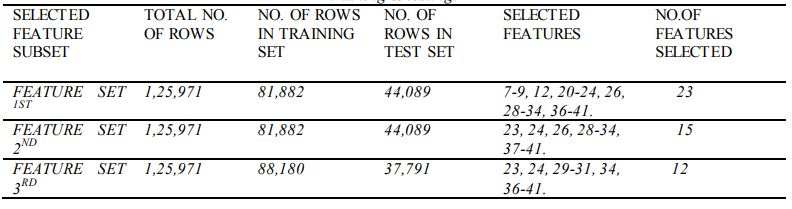
\includegraphics[width=80mm]{Gambar/gambar1.JPG}}
\captionof{figure}{Menunjukkan subset fitur yang dipilih dan jumlah instance yang dipilih secara acak dari Dataset NSL-KDD untuk pelatihan & pengujian}
\label{fig2}
\end{minipage}

\subsection{Classification}
Tantangan utama yang dihadapi IDS adalah False Alarm (negatif palsu dan positif palsu) dan kekurangan dari respon waktu nyata. Algoritma pembelajaran mesin memiliki kekuatan untuk mengatasi tantangan seperti itu. Mesin teknik pembelajaran dapat digunakan untuk membangun kecerdasan IDS yang dapat mendeteksi baik yang diketahui maupun yang tidak diketahui serangan dengan kecepatan tinggi, akurasi maksimum dan tingkat alarm palsu minimum\cite{masoodi2019symmetric}\cite{jabbar2017rfaode}. Jadi mesin algoritma pembelajaran dapat digunakan untuk meningkatkan IDS dengan kemampuan yang ditingkatkan. pengklasifikasi pembelajaran mesin, yaitu RF (Random Forest), DT (Decision Tree), MLP (Multi-layer Perceptron), dan SVM (Dukungan Vector Machine) digunakan sebagai pemantau intrusi mesin untuk menemukan intrusi dengan mengklasifikasikan data. Hutan acak adalah pembelajaran terawasi yang kuat algoritma. Random Forest adalah pengklasifikasi ensemble (terdiri dari multiple decision tress) yang digunakan untuk meningkatkan kinerja sistem\cite{rutkowski2012decision}. Itu output dari beberapa pohon dipilih untuk mengkategorikan data di kelas yang sesuai. Random Forest paling banyak menggunakan algoritma pembelajaran mesin yang diawasi untuk pengelompokan, klasifikasi data berdasarkan kesamaan fitur yang mereka bagikan. Hutan Acak dibangun dari pohon yang terbatas. Setiap pohon berperilaku seperti satu keputusan pohon di mana setiap pohon memilih fitur secara acak dari Himpunan data. Oleh karena itu, Menggunakan Pohon Acak untuk tujuan klasifikasi, jumlah pohon harus diperbaiki sebelum implementasi. DT adalah pembelajaran mesin algoritma klasifikasi untuk mengklasifikasikan data. Itu algoritma pohon keputusan secara predikatif dipelajari untuk membangun model dari kumpulan data yang dikategorikan ke memetakan sebuah instance berdasarkan serangkaian fitur yang dipilih ke kelas tertentu\cite{alsmadi2017sdn}. Setiap sampel ditentukan oleh nilai-nilai mereka dari fitur masing-masing. Fungsi utama adalah untuk mendeteksi fitur, yang paling baik membagi data ke dalam kelasnya masing-masing. Node dapat dibagi dengan menggunakan entropi. Entropi mengukur kemurnian pemisahan sampel dalam simpul. Untuk tujuan membagi entropi digunakan dalam penelitian ini untuk memilih node terbaik. MLP (Multilayer Perceptron) adalah jaringan saraf terdiri dari satu atau lebih dari satu lapisan tersembunyi. Lapisan dalam MLP harus minimal tiga lapisan yaitu input, output dan lapisan tersembunyi yang memetakan variabel masukan menjadi keluaran akhir\cite{sain1996nature}. Diperbaiki fungsi unit linier digunakan untuk melatih dan menguji model dan 10 neuron digunakan hanya di hidden lapisan. SVM adalah algoritma pembelajaran terawasi yang digunakan untuk kategorisasi biner dari non linier dan linier data. SVM (Support Vector Machine) mengklasifikasikan: data dengan membangun hyperplane N-dimensi dengan membagi sekelompok sampel positif dari sekelompok sampel negatif dengan margin tertinggi \cite{yang2015evaluating}\cite{sain1996nature}.Untuk pelatihan fungsi kernel basis radial diterapkan untuk memaksimalkan hasil prediksi untuk data non-linear. Kinerja model yang diusulkan adalah dianalisis pada tiga subset fitur berbeda yang diekstraksi dari kumpulan data NSL-KDD. Pra-pemrosesan adalah tugas penting untuk menghapus/mengganti fitur yang tidak relevan untuk meningkatkan akurasi dan meningkatkan ketahanan dari proses deteksi. Penampilan, biaya komputasi IDS didasarkan pada fitur/dimensi yang dipilih dari dataset, oleh karena itu, kumpulan data telah diproses sebelumnya untuk dihapus atribut yang tidak penting. Dalam penelitian ini bekerja dua dataset digunakan. Fitur-fitur yang berkontribusi yang paling untuk klasifikasi dipilih secara acak.

\section{Results}
Percobaan dilakukan pada dataset NSL-KDD. Dataset NSL-KDD memiliki 41 kolom, membuatnya sulit untuk bekerja karena mereka meningkatkan biaya komputasi. Oleh karena itu, dataset direduksi untuk memenuhi persyaratan untuk percobaan. Tiga set data adalah dipilih secara acak dari dataset asli untuk mengurangi biaya komputasi. Semua percobaan adalah dilakukan di Google Colab dan efektivitas semua pengklasifikasi dalam mengklasifikasikan kumpulan data NSL-KDD adalah dipelajari. Pengklasifikasi RF menghasilkan yang tertinggi akurasi di atas 99 persen menggunakan subset fitur pertama. Random Forest adalah teknik klasifikasi ensemble (beberapa pengklasifikasi digabungkan untuk meningkatkan prediksi) yang menggunakan bilangan berhingga (dua atau lebih) pohon keputusan untuk melakukan klasifikasi. Jadi model mengurangi biaya komputasi dengan menghapus beberapa fitur yang tidak relevan dan meningkatkan akurasi model terutama untuk RF dan DT. Tabel 2 menunjukkan hasil pengklasifikasi yang berbeda di mengklasifikasikan data menggunakan tiga yang dipilih secara acak subset fitur dan gambar 1 menunjukkan grafik representasi temuan dalam hal akurasi pada berbagai subset fitur.

\begin{minipage}{\linewidth}
\centerline{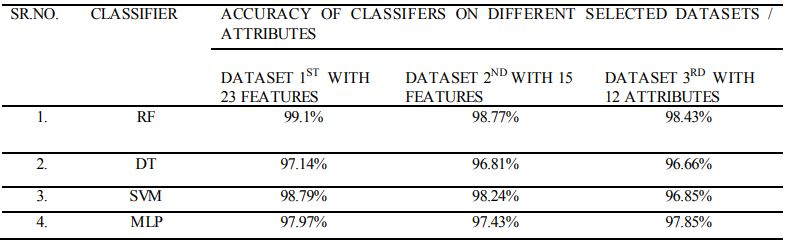
\includegraphics[width=80mm]{Gambar/gambar2.JPG}}
\captionof{figure}{Hasil yang dihasilkan oleh empat pengklasifikasi (RF, DT, SVM, MLP) pada tiga set data dengan set fitur yang berbeda}
\label{fig2}
\end{minipage}

\begin{minipage}{\linewidth}
\centerline{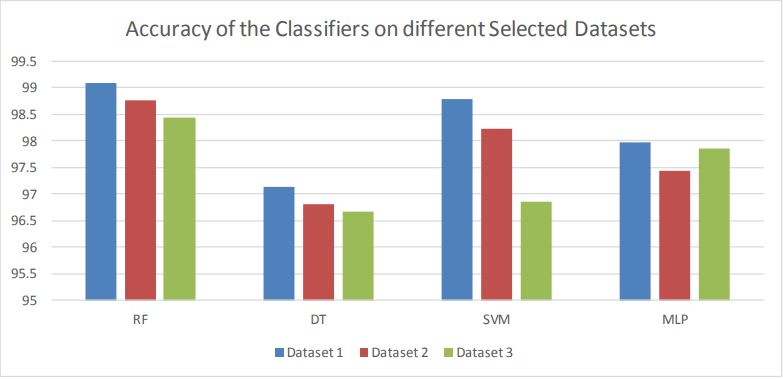
\includegraphics[width=80mm]{Gambar/gambar3.JPG}}
\captionof{figure}{Representasi grafis dari hasil yang dihasilkan}
\label{fig2}
\end{minipage}

\section{Kesimpulan}

Dalam makalah ini, eksperimen empiris dilakukan menggunakan empat pengklasifikasi pembelajaran mesin yaitu RF, DT, MLP, dan SVM untuk menguji dan menguji efisiensi dan kinerja. Pelatihan dan penguji dilakukan pada tiga subset fitur yang diekstraksi dari set data deteksi intrusi NSL-KDD. Mulanya Dataset NSL-KDD telah dibawa sebelumnya untuk memilih fitur yang relevan untuk meningkatkan efisiensi dan mengurangi waktu pelatihan. Dalam Percobaan 81.882 kasus baris yang digunakan untuk melatih mesin yang dipilih model pembelajaran. Untuk tujuan pengujian 44.089 acak contoh yang digunakan. hasil berdasarkan yang dicapai hutan acak menghasilkan tingkat klasifikasi tertinggi lebih dari 99 persen, dan pohon keputusan menghasilkan tingkat akurasi terendah 96,60 persen di antara empat pengklasifikasian. Para peneliti harus fokus pada positif palsu dan kinerja negatif negatif yang menurunkan kinerja model deteksi intrusi. itu studi empiris telah mengungkapkan bahwa tidak ada pembelajaran mesin yang dapat mendeteksi semua bisa jenis serangan secara efektif. Di masa depan, relevan fitur dapat diekstraksi dari dataset asli untuk mengurangi waktu dan meningkatkan tingkat akurasi pengklasifikasi pembelajaran mesin. Metode berbasis ensemble dapat digunakan untuk menguji dan kinerja, metode ini dapat memprediksi serangan secara efisien.

\bibliographystyle{IEEEtran}
\bibliography{referensi.bib}

\end{document}
